\section{Constraint-aware Optimization}
\label{sec:optimization}

\begin{figure*}[pos=tbp]
    \centering % 将图居中
    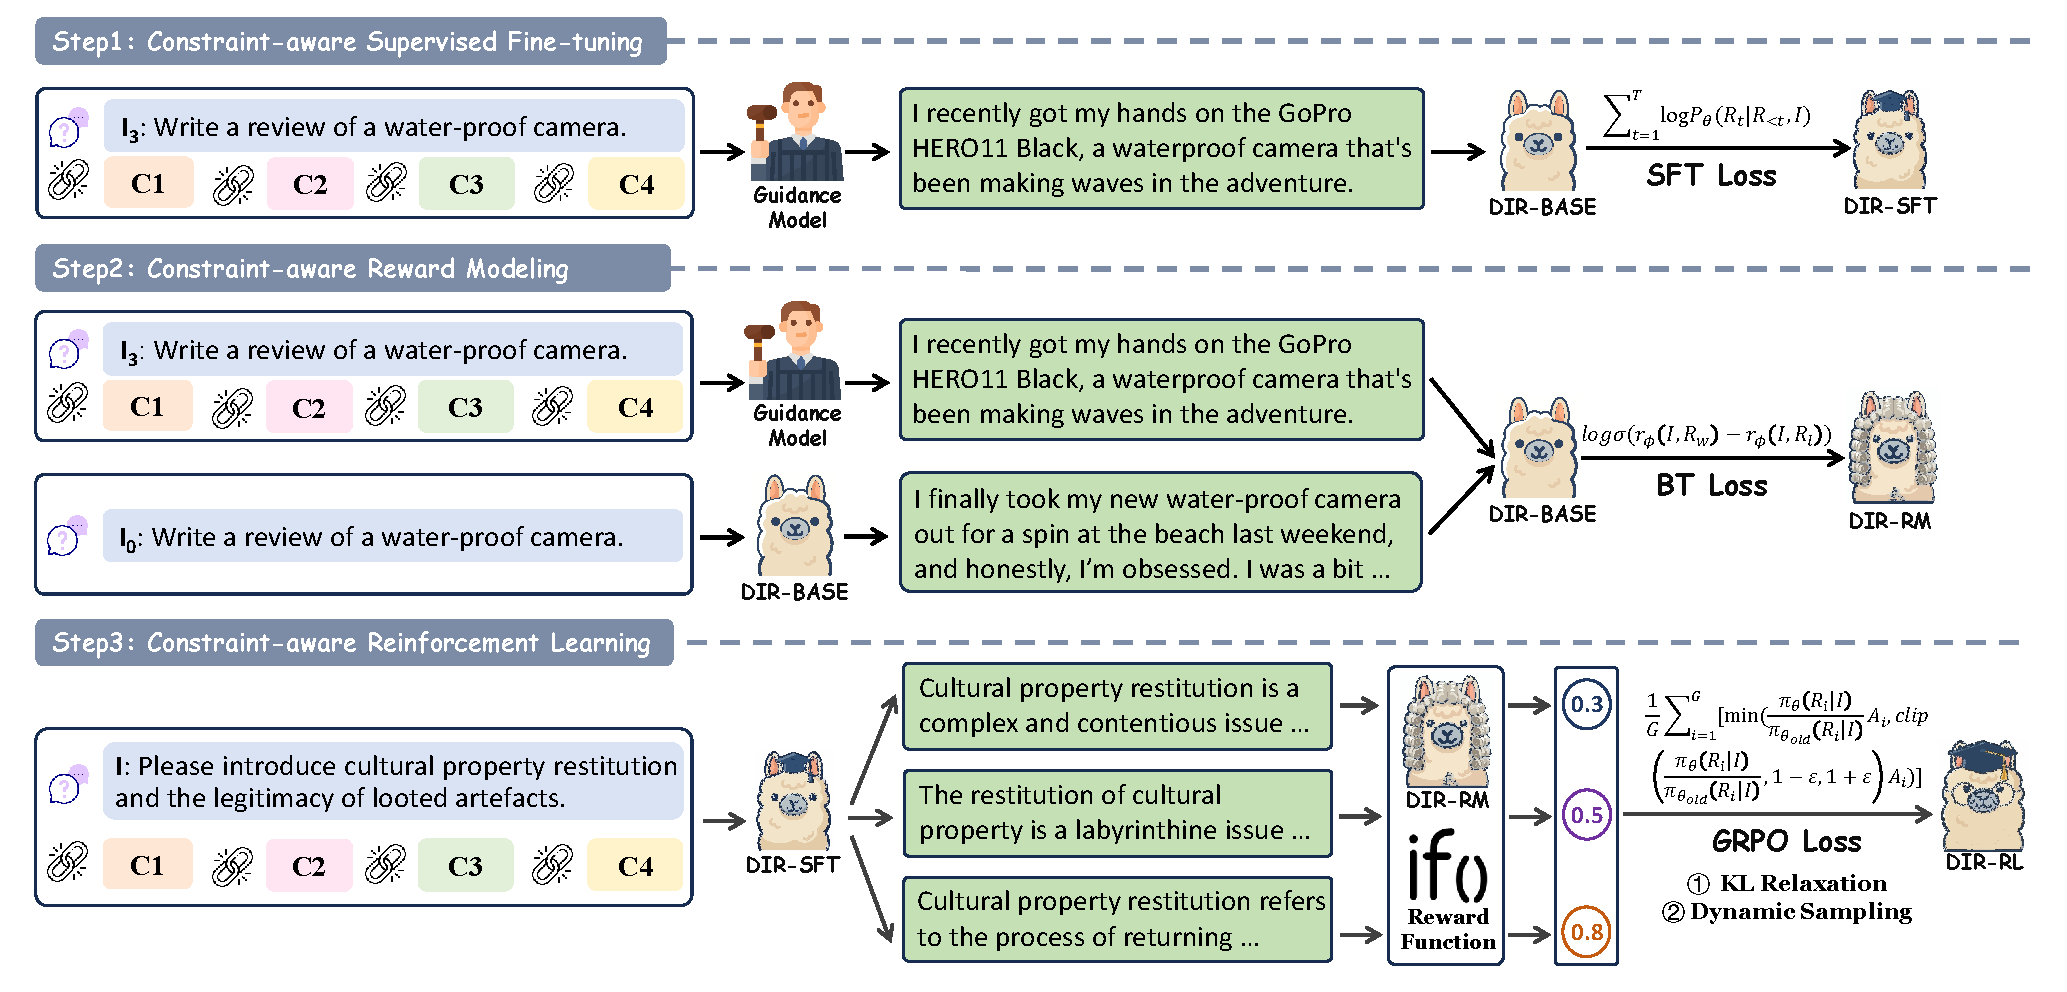
\includegraphics[width=1.0\linewidth]{source/main_RL.pdf}
    \caption{
     The Illustration of Constraint-aware Optimization. We first perform Constraint-aware SFT on responses curated by the guidance model. Then we leverage intermediate responses generated during the iterative process as negative samples, to train the Constraint-aware Reward Model (RM). Finally, we conduct Constraint-aware Reinforcement Learning, guided by a hybrid feedback mechanism that integrates both the neural RM and rule-based rewards.
    }
    \label{fig:main_rl}
\end{figure*}

Building upon the high-quality instruction data \textbf{DIR-10K}, we present a constraint-aware optimization pipeline to enhance the instruction-following capabilities of LLMs, as illustrated in Figure \ref{fig:main_rl}. This method mainly consists of two steps, as in the following sections.

\subsection{Constraint-aware Supervised Fine-tuning}

The first stage involves Supervised Fine-Tuning (SFT) \citep{ouyang2022training} using the standard negative log-likelihood (NLL) loss:

\begin{equation}
\begin{aligned}
\mathcal{L}_{SFT}(\theta) & = \\
& \quad -\sum_{t=1}^{T} \log P_{\theta}(R_t \mid R_{<t}, I)
\end{aligned}
\end{equation}

\noindent where $I$ represents the complex instruction and $R$ denotes the curated response. Since our instructions are iteratively refined to incorporate diverse real-world constraints, this stage enables the model to establish a foundational mapping between complex instructions and desired outputs.

Notably, while the refined document serves as the basis for the judgment process, it is not used as the target for fine-tuning, as the document itself may not explicitly align with the newly introduced constraints~\citep{nguyen2024better}. Instead, we leverage the guidance model to generate responses based on the combined instructions, ensuring that the model is optimized on responses that strictly adhere to the specified constraints.

\subsection{Constraint-aware Reinforcement Learning}
\label{sec:rl}

While SFT effectively initiates the model with complex instruction-following capabilities, it faces three critical bottlenecks: \textbf{1) Lack of Negative Supervision:} SFT focuses solely on maximum likelihood estimation of positive samples, failing to provide the explicit penalties necessary to suppress undesirable behaviors \citep{gudibande2023falsepromiseimitatingproprietary}. This prevents the model from associating constraint violations with performance degradation. \textbf{2) Teacher-bounded Performance:} The model's performance is inherently capped by the quality of the reference response generated by the guidance model. This restricts the model from exploring more optimal response strategies that might surpass the teacher's initial output. \textbf{3) Sparse Reward Signals:} Many complex constraints (e.g., inclusion constraint, length constraint) are discrete and non-differentiable, making them ill-suited for SFT’s token-level cross-entropy loss.

To bridge these gaps, we propose constraint-aware Reinforcement Learning (RL) that transitions from pattern imitation to direct constraint alignment. The RL is based on a hybrid reward system as follows.

\subsubsection{Model-based Reward}

For subjective constraints such as sentiment and tone, we train a discriminative reward model $r_\phi$ using the Bradley-Terry objective:

\begin{equation}
\begin{aligned}
\mathcal{L}_{RM}(\phi)
&= -\mathbb{E}_{(I, R_w, R_l) \sim \mathcal{D}_{pref}}
\left[ \log \sigma \left( r_\phi(I, R_w) \right.\right. \\
&\hspace{5.7em}\left.\left.{} - r_\phi(I, R_l) \right) \right]
\end{aligned}
\end{equation}

\noindent where $R_w$ and $R_l$ are the chosen and rejected responses.

We leverage the iterative nature of the DIR framework to construct high-quality preference pairs $(I, R_w, R_l)$. As shown in Algorithm \ref{alg:iir}, during the IIR process, the guidance model identifies specific deficiencies in the response from a previous iteration ($R_i$) and proposes incremental constraints to rectify them. Consequently, $R_i$ naturally serves as the rejected sample $R_l$, while the refined response from the guidance model acts as the chosen sample $R_w$. By training on these pairs, the reward model effectively internalizes instruction following and learns to assign higher scores to responses that satisfy sophisticated constraints.
%, thereby providing a robust guidance signal for the subsequent RL process.

To mitigate the potential degradation of general capabilities during reinforcement learning, we augment the preference data with samples from the \textit{Skywork-Reward-Preference-80K-v0.2} dataset \citep{liu2025skywork} at a 1:1 ratio. This balanced mixture ensures that the reward model maintains a robust assessment of both general and complex instruction alignment.

\subsubsection{Rule-based Reward}
For verifiable hard constraints (e.g., length, keyword inclusion), we employ automated scripts to generate a binary signal $V(\mathbf{c}, R) \in \{0, 1\}$, where $\mathbf{c}$ denotes the set of hard constraints specified in $I$. To prioritize these hard constraints over stylistic nuances, we implement a Constraint-prioritized Reward Fusion strategy:

\begin{equation}
\mathcal{R}(I, R) =
\begin{cases}
\sigma(r_\phi(I, R)) & \text{if } \mathbf{c} = \varnothing \\
0.5 + 0.5 \cdot \sigma(r_\phi(I, R)) & \text{if } V(\mathbf{c}, R) = 1 \\
0.5 \cdot \sigma(r_\phi(I, R)) & \text{if } V(\mathbf{c}, R) = 0
\end{cases}
\end{equation}

This piecewise mapping ensures that any response failing hard constraints ($V=0$) receives a strictly lower score (range $[0, 0.5]$) than those satisfying them ($V=1$, range $[0.5, 1.0]$).

\subsection{Optimization with GRPO}

Based on the hybrid reward system, we utilize Group Relative Policy Optimization (GRPO) \citep{shao2024deepseekmath} to perform RL. To better adapt GRPO to complex instruction-following tasks, we introduce two key modifications:

\begin{enumerate}[leftmargin=4mm]
    \item \textbf{KL-Penalty Relaxation:} Unlike traditional RLHF where RL objectives may diverge from the SFT distribution, our SFT and RL stages share the unified goal of instruction following, and the risk of representation collapse is significantly reduced \citep{parthasarathi2025grpolambdacreditassignmentimproves}. Therefore, we omit the explicit KL-penalty term from the loss function, relying instead on the PPO-style clipping mechanism for stability \citep{hu2025openreasonerzeroopensourceapproach}. This relaxation allows for more aggressive exploration and closer alignment with complex constraints.
    \item \textbf{Dynamic Sampling Mechanism:} As the policy optimizes, standard uniform sampling frequently encounters saturated groups where all responses satisfy the constraints, resulting in uninformative reward differences \citep{yu2025dapo}. To maintain optimization efficiency, we implement a mechanism that evaluates the within-group reward standard deviation, and if the deviation falls below a predefined threshold $\tau$, the query is identified as lacking sufficient discriminative signal and is dynamically excluded from the optimization step.
\end{enumerate}

Based on the two modifications, the optimization objective during our RL phase is as follows:

\begin{equation}
\begin{split}
\mathcal{L}_{GRPO}(\theta) & = \frac{1}{G} \sum_{i=1}^{G} \bigg[ \min \Big( \frac{\pi_{\theta}(R_i|I)}{\pi_{\theta_{old}}(R_i|I)} \mathcal{A}_i, \\
& \text{clip}\left( \frac{\pi_{\theta}(R_i|I)}{\pi_{\theta_{old}}(R_i|I)}, 1-\epsilon, 1+\epsilon \right) \mathcal{A}_i \Big) \bigg]
\end{split}
\end{equation}

\noindent where for each instruction $I$, we sample a group of outputs $\{R_i\}_{i=1}^G$, and the advantage $\mathcal{A}_i$ is computed by normalizing the rewards $\mathcal{R}(I, R_i)$ within the group:

\begin{equation}
\mathcal{A}_i = \frac{\mathcal{R}(I, R_i) - \text{mean}(\mathcal{R}(I, R_1), \dots, \mathcal{R}(I, R_G))}{\text{std}(\mathcal{R}(I, R_1), \dots, \mathcal{R}(I, R_G))}
\end{equation}

By incorporating explicit penalties for constraint violations, the RL framework provides a holistic evaluation signal that enables the model to distinguish between compliant and non-compliant responses, thereby enhancing its instruction following ability for both general and complex instructions.